\section{Measurement study and Key metrics prediction}\label{sec:prediction}
In \autoref{subsec:ltenet} we show in proportional fair scheduler the available bandwidth for each user is a function of (i) number of users in each cell, and (ii) the channel quality for each user, so the predictability of the two determines the estimated bandwidth. In this section we conduct an extensive measurement study to show the predictability of the link channel quality and the load on eNodeBs in \autoref{subsec:Prediction}. 

The traces are collected in Jun and July 2014 over several geolocations in the United States from one major 4G network carrier, it covers more than half million users and over 2000 eNodeBs. The traces have been anonymized before handing to us for privacy reasons. 

\subsection{Proportional Fair Scheduler}\label{subsec:ltenet}
3G ad 4G networks are using Orthogonal Frequency-Division Multiuser Access(OFDMA) scheme to achieve high spectrum efficiency. To achieve multiuser diversity, NodeBs and eNodeBs are running variations of proportional fair scheduling system. A basic \textit{proportional fair scheduler} works as the following: eNodeBs obtain the feedback from each user about their instantaneous channel quality conditions (CQ) in terms of encoding rate per resource block, and take the ratio between it and historical mean of CQ and pick the user with the maximum ratio. In a static model over a long term, each user will get 1/N share of resource blocks if N is the static number of users in the cell, a dynamic model also has a similar result\cite{PFINFOCOM}. The maximum bandwidth for each user in a cell is a function of: $T$-number of resource blocks in the cell, $N$-number of users in the cell, and $\mathbf{CQ}$-channel quality vector for all users; so maximum bandwidth vector for all users $\mathbf{BW} = f(T, N, \mathbf{CQ})$. We do not directly address $f(T, N, \mathbf{CQ})$ function in this paper as it is a vendor-specific PF-based scheduler. In the rest of the paper we assume a simple PF scheduler model, that is $\mathbf{BW} = f(T, N, \mathbf{CQ})=\frac{T}{N}*\mathbf{CQ}$. Among the three variables, $T$ is predetermined by the hardware, $N$ and $\mathbf{CQ}$ are the two factors we need to predict. 

\subsection{Bandwidth Estimation} \label{subsec:Prediction}


\subsubsection{Predictability}
First we define criteria for predictability: (1) Mean Absolute Percentage Error (MAPE); and (2) $\sum\text{MPE}_t$; where MPE stands for Mean Percentage Error. The reason for (1) is to minimize the side effect it gives to the video streaming application for each prediction it makes, and the reason for (2) is to avoid a biased prediction. For our domain specific application, (2) is especially important since (i) short term prediction error can be absorbed by the client playback buffer, and (ii) long term prediction should compensate the short term error, i.e., we can underestimate at time t and overestimate at time t+1 and the two errors are offset in application decision making. 


\subsubsection{Cell Load}\label{subsec:NUser}
We measured the number of active users in each cell from the same trace as mentioned above. The trace is collected from UE's RSRQ reports to eNodeBs. In a simple model if a user reports RSRQ in a one-second interval, we assume that user is active in that second. 

\begin{figure}[t]
\centering
 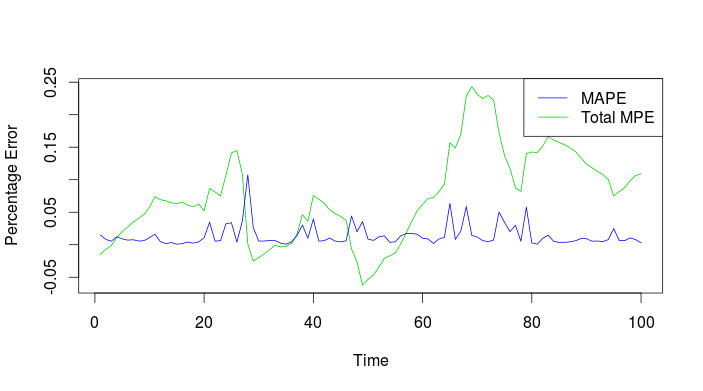
\includegraphics[width=0.8\linewidth]{pictures/MPE.png}
\caption{Error Analysis for Cell Load} \label{fig:NAIVEMPE}
\end{figure}

Although we predict the number of active users, we use the inverse value to compute the available bandwidth so MAPE=$ |\frac{1}{N_{true}} - \frac{1}{N_{pred}}| *N_{true}$, and $\text{MPE}_t=(\frac{1}{N^t_{true}} - \frac{1}{N^t_{pred}})*N^t_{true}$. ARIMA (auto-regressive integrated moving average) model can predict the number of active users with a fair accuracy, as it fits well with a stochastic model. We use auto.arima function in R ``forecast'' package to fit the best ARIMA model, and set the sliding time window to 15 seconds in both here and the following section. In fact for a moderate to heavy loaded cell a random walk, or ARIMA(0,1,0) occurs the most often. 

We plot MAPE and total MPE for one cell in a two minutes span in \autoref{fig:NAIVEMPE}, as we can see that the prediction has fairly small miscalculation at each step, and the total MPE $\sum$MPE$_t$ may oscillate to a greater positive or negative value. 
\begin{figure}[t]
\centering
 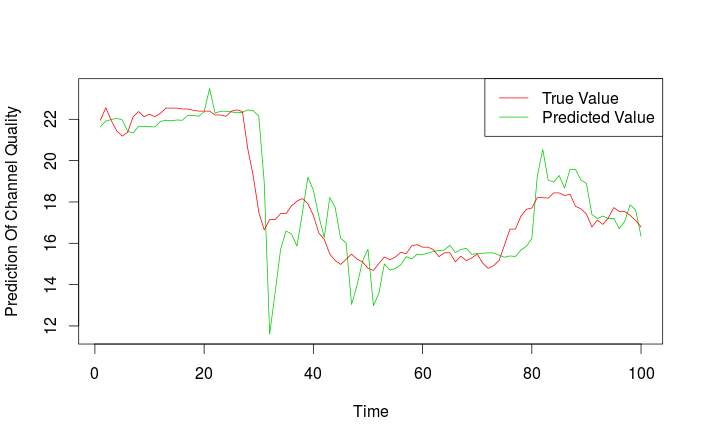
\includegraphics[width=0.8\linewidth]{pictures/prediction.png}
\caption{One sample prediction for channel quality: the algorithm makes a conservative estimation for channel quality once  it detects a great overestimation at 30s to minimize the total error} \label{fig:prediction}
\end{figure}
\subsubsection{Channel Quality}\label{subsec:CQ}
One unique characteristic for cellular network is the high mobility and this causes the link quality to fluctuate to a certain extent.

\emph{RSRQ:} Reference Signal Received Quality, is the key metric for the LTE wireless channel. RSRQ senses the load from other users in the same cell and the neighboring cells, and is indexed in 0-34 integer numbers; a higher number indicates a better link quality. RSRQ values can be mapped to certain encoding rate.
\begin{comment}
\emph{Data characteristic:} we find most of the users have fairly stable link quality, 54.6\% of the users have a CV (co-efficiency of variation) in terms of RSRQ within 0.2, but 3.6\% of the users have very dynamic link with a CV higher than 1. \emph{The Occurrence of Handoff}: in the dataset, handoff occurs for 30.7\% of the users, and average handoff occurrence is 2.2 times. Through further investigation, we found repetitive switch between two or three neighboring cells is quite often in our dataset, mostly due to similar RSRQs ($\Delta RSRQ<5$) from both cells. 
\end{comment}

Unlike Cell Load, the channel quality pattern is constantly switching between different ARIMA models when we apply auto.arima, and the prediction may keep over or under-estimating, in other words, the prediction may be biased. To address this problem, we add an auto-adjustment in prediction algorithm to keep the total error small. 

Through replay 50 random traces where the UEs are active for more than 100 seconds, we found that MAPE$<0.2$ for almost all the users, but $\sum\text{MPE}>0.5$ is in fact quite often. Without our auto-adjustment, $\sum\text{MPE}>1$ can also happen. 

The above results give us great insights in terms of prediction accuracy: a prediction can be 80\% accurate for each time segment while the cumulative error can be as much as 50\% of one time segment's bandwidth. 










\begin{comment}

\section{Design} \label{sec:optimization}
In this section, we explain the reason to choose an \textbf{\emph{end-to-end decision making with in-network knowledge}} model in section \ref{designchoice}, we then explain the our architecture in section \ref{architecture}. 
%introduce performance metrics in section \ref{metrics} and 

\subsection{Who decides the video streaming?}\label{designchoice}
For video streaming service decision making, there are three different models: \emph{In-network}, \emph{strictly end-to-end} and \emph{End-to-end with in-network knowledge}. 

\emph{In-network techniques} make decisions for users: it selects the video bit rate and schedule the download for users based on its knowledge of the network condition. However in-network approaches lack the insight of the video play progress, e.g., video buffer occupancy since it does not deal with any video decoding. Aside from technical reasons, here are several privacy/policy reasons for not doing this: most content providers are using encrypted http connections which ISPs cannot access; users may be concerned about their data budgets and thus not choose high bit rate; or content providers have different video play bit rate policies for different users based on their subscription contracts. 

\emph{End-to-end techniques} probe the network condition based on round trip time (RTT) and historical throughput, however existence of the proxy makes the RTT very inaccurate as it splits tcp connections. The dynamic nature of the wireless link makes historical data unable to capture the link behavior, e.g. the available bandwidth may plummet due to fading effects or handoff and recovers very soon after, current end-to-end approaches fail to react to those scenarios in most cases.

\emph{End-to-end with in-network knowledge} model addresses the above issues: instead of making the decision for the client; the network helps video streaming service make better decisions via offering some key performance metrics about the network condition, such as available throughput and handoff. 

Though an end-to-end with in-network knowledge approach has advantages over the other two, we still need to address the problem of how to expose the in-network knowledge in a least intrusive way in a scalable manner. 







\subsection{Architecture}\label{architecture}

We propose a two-tiered system for to implement OpenCell system. The two parts sit in RAN and EPC respectively. 

At the lower tier we have bandwidth estimator for each eNodeB. Estimating link channel quality and cell load is much more scalable if if we compute it at eNodeBs, since there are only hundreds of users at each cell, while aggregated number of users for a SGW can be tens of thousands. Making an estimation at second level means for each user the computational cycle is ~1 $ms$ if sitting at eNodeBs and ~10  $\mu s$ if sitting at Serving Gateway. Processing the raw information such as RSRQ from eNodeBs and extract it as estimated bandwidth also reduces the extra traffic generated for message passing. 

At the higher tier, the information inferred at eNodeBs are received at the proxy, and combined with handoff information, we make a final estimation of available bandwidth for each user and then expose this piece of information to application service providers by some means. The architecture is in figure \ref{cellular}.

\begin{figure}[t]\label{cellular}
\begin{minipage}[b]{\linewidth}
\centering
 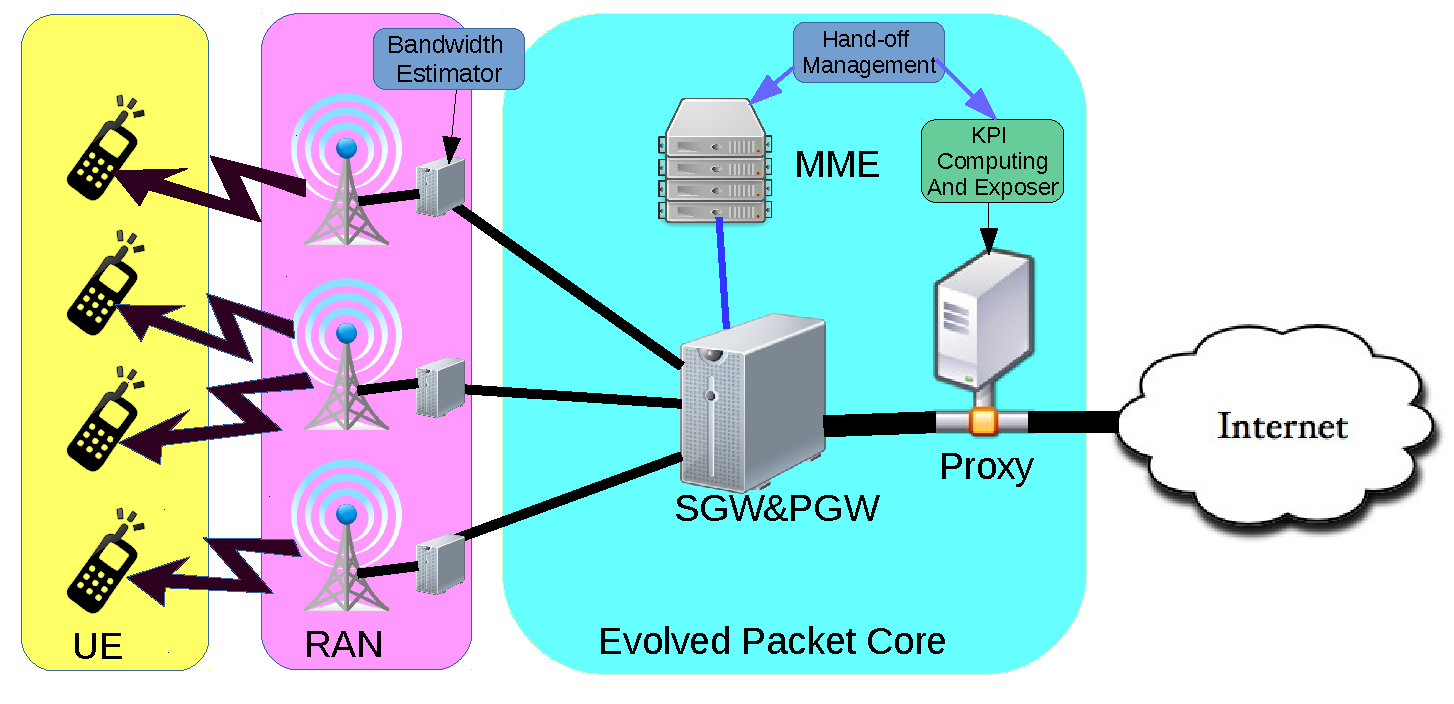
\includegraphics[width=\linewidth]{cellular.pdf}
\end{minipage}
\caption{OpenCell Design}
\end{figure}

In terms of how to expose the API information, there are three options: encapsulation (i) at TCP/IP layer, (ii) at application layer; and (iii) using a distinct channel. Each approach has its pros and cons, for example TCP/IP layer does not require DPI but the fields used for encapsulation might be overwritten deep in the network from middleboxes. Using distinct channel does not suffer either problem but it requires application service providers' cooperation. We are still weighing between the options and leave this as a future problem. 



\end{comment}
